\documentclass[a4paper,10pt]{article}
\usepackage[T1]{fontenc}
\usepackage[english]{babel}
\usepackage{mathtools}
\usepackage{bbm}
\usepackage{amsmath}
\usepackage{amsfonts}
\usepackage{amssymb}
\usepackage{fancyhdr}
\usepackage{geometry}
\usepackage{subfig}
\usepackage{enumerate}
\usepackage{graphicx}
\usepackage{caption}
\usepackage{subfig}
\usepackage{tabu}
\usepackage{multirow}
\usepackage{color}
\usepackage{listings}
\usepackage[]{algorithm2e}
\usepackage[autostyle,english=british]{csquotes}
\usepackage{minitoc}

\newtheorem{thm}{Theorem}
\newtheorem{defn}{Definition}
\newtheorem{prop}{Proposition}

%opening
\title{Monte Carlo solvers for sparse linear systems}
\author{Michele Benzi, Massimiliano Lupo Pasini}
\date{}

\begin{document}

\maketitle

\begin{abstract}
We consider linear systems of equations characterized by a sparsity pattern,
focusing in particular on problems derived from the discretization of partial
differential equations. We propose a treatise of the current stochastic
techniques present in literature that might be employed to solve the problems at
hand. New theoretical results are introduced as sufficient criteria for the
guarantee of the convergence of the methods analyzed. An analysis about viable
preconditioners is accomplished as well.
\end{abstract}

\section{Introduction}
\label{sec:intro}

For a long period the
pursuit of a reliable solver for linear and nonlinear algebraic systems has
been one of the most important issues in Numerical Analaysis. The
mathematical properties of the model (e.g. likely sparsity pattern of the
matrix) have urged scientists to look for efficient and pattern-driven
solvers, capable to cope with curse of dimensionality and high scalability
requests.

As scalability computing move towards exascale facilities (which stands for
machines computing up to $10^{18}$ flops), new numerical schemes suitable for
this
kind of architectures are strongly demanded. In fact the purpose is to combine
high
fidelity of the results with an optimized use of hardware resources at hand.

Recently new algorithms that combine statistical and numerical techniques have
been developed. Even though \textit{numerical efficiency} has been sacrificed
sometimes, the advantages in terms of \textit{robustness} of these methods make
it worth carrying on studies in this direction.
A class of methods that may be employed for this purpose is represented by
Monte Carlo linear solvers.

These algorithms are the main topic covered in the work presented here,
starting from what was developed so far by some of
the authors who gave significant contributions (see \cite{Hal1962},
\cite{Hal1994},
\cite{DA1998}, \cite{DVA2001}, \cite{AADBTW2005},\cite{ESW2013} and
\cite{EMSH2014}). \newline

As underlined in \cite{DA1998}, Monte Carlo methods may be split into two
classes: \textit{direct methods} (\cite{DA1998}, \cite{DVA2001}) and
\textit{iterative methods} (\cite{Hal1962},
\cite{Hal1994}, \cite{ESW2013}
and \cite{EMSH2014}). The first are characterized by a merely stochastic
scheme,
therefore the provided error with respect to the exact solution is made of
just a stochastic component. The iterative Monte Carlo methods utilize more
traditional iterative algorithms alongside the stochastic approach,
generating two types of error: a
\textit{stochastic} one and a \textit{systematic} one. It does not
mean
that
it will be always simple to recognize them separately. However it is important
to
be
aware of this intrinsic structure, in order to target what is the part of the
scheme that requires a refinement (e.g. increasing the number of iterations
rather than the number of random walks).

The paper is organized as follows.
In Section~\ref{sec:mcls} we provide an overview of existing Monte Carlo
linear solver algorithms.
In Section~\ref{sec:convergence} we will discuss the convergence behavior
of stochastic solvers, including a discussion of classes of matrices for
which convergence can be guaranteed.
Section~\ref{sec:results} provides some numerical results illustrating
pertinent properties of the various approaches and Section~\ref{sec:conclusion}
will provide some concluding remarks and areas for future investigation.


\section{Stochastic Linear Solvers}
\label{sec:mcls}

We consider the solution of systems of linear equations of the form
\begin{equation}
A \mathbf{x}=\mathbf{b},
\label{linsys}
\end{equation}
where $A\in \mathbb{R}^{n\times n}$ and $\mathbf{x}$, $\mathbf{b} \in
\mathbb{R}^n$.

Equation~(\ref{linsys}) can be reinterpreted as a fixed point scheme
\begin{equation}
 \mathbf{x}=H\mathbf{x}+\mathbf{f}.
 \label{fixedpoint}
\end{equation}
where $H=I-A$ and $\mathbf{f}=\mathbf{b}$.

Assuming that the spectral radius $\rho(H)<1$, the solution to
(\ref{fixedpoint}) can be written in terms of a power series of
$H$ (Neumann series)
\[
\mathbf{x}=\sum_{i=0}^\infty H^i\mathbf{f}.
\]
Therefore the fixed point scheme generates a sequence of approximate solutions
$\{\mathbf{x}^{(k)}\}_{k=0}^{\infty}$ which converges to the exact solution
regardless of the initial guess $\mathbf{x}_0$.

By restricting the attention to a single component of $\mathbf{x}$ we
have
\begin{equation}
x_i=\sum_{\ell=0}^\infty \sum_{k_1}^n\sum_{k_2}^n\cdots \sum_{k_{\ell}=1}^n
H_{k_0,k_1}H_{k_1,k_2}\cdots H_{k_{\ell-1}, k_{\ell}}f_{k_{\ell}}.
\label{forward}
\end{equation}
The last equation can be reinterpreted as the realization of an estimator
defined on a random walk.  Let us start considering a random walk whose
state space $S$ is characterized by the set of indices of the forcing term
$\mathbf{f}$:
\[
S=\{1,2,\cdots, n\} \subset \mathbb{N}.
\]
Each $i$-th step of the random walk has a random variable
$k_i$ associated with it. The realization of $k_i$ represents the index of the
component of $\mathbf{f}$
which is visited in the current step of the random walk.
The method of building the transition probabilities and the selection of
the initial state of the random walk gives rise to two different approaches:
the \textit{forward} and \textit{adjoint} methods.

\subsection{Forward Method}
\label{subsec:forward}

The goal is to evaluate a functional such as
\[
J(\mathbf{x})=(\mathbf{h},\mathbf{x})=\sum_{i=1}^n h_i x_i.
\]
where $\mathbf{h}\in \mathbb{R}^n$ is the Riesz representative in
$\mathbb{R}^n$ of the functional $J$.
We can use it to build the initial probability $\tilde{p}:
S\rightarrow [0,1]$ of the random walk such that
\[
\tilde{p}(k_0=i)=\tilde{p}_{k_0}=\frac{\lvert h_i\rvert}{\sum_{i=1}^n \lvert
h_i\rvert}.
\]
It is important to stress out that the role of vector $\mathbf{h}$ is
restricted to the construction of the initial probability and is not
used further in the definition of the stochastic process.
A possible choice for the transition probability $P$ can be
\[
p(k_i=j \;\lvert\;k_{i-1}=i )=P_{i,j}=\frac{\lvert H_{i,j}\rvert}{\sum_{k=1}^n
\lvert H_{i,k}\rvert}.
\]
where $\tilde{p}(\cdot,i):S\rightarrow [0,1]$ $\forall i\in S$.
A related sequence of random variables $w_{i,j}$ can be defined
such that
\[
w_{i,j}=\frac{H_{i,j}}{P_{i,j}}.
\]
The probability distribution of the random variables $w_{i,j}$ is represented
by the transition matrix that rules the stochastic process. The $w_{i,j}$'s
just introduced can be used to build one more sequence
of random variables.
At first we introduce quantities $W_j$
\[
W_{0}=\frac{h_{k_0}}{\tilde{p}_{k_0}}, \quad W_j=W_{j-1} w_{i,j}, \quad
j=1,\cdots, i.
\]
By defining
\[
X(\nu)=\sum_{m=0}^k W_m f_{i_m}
\]
as the random variable associated with a specific permutation $\nu$, we can
define the estimator $\theta_i$ such as
\[
\theta=E[X]=\sum_{\nu}P_{\nu}X(\nu).
\]
The integer $n$ represents the size of the solution vector to (\ref{linsys})
and
the
index
$i$
is referred to the component of the solution vector we want to compute.
$P_{\nu}$ is the probability associated with a specific permutation of the
random walk.
It can be proved that
\[
E[W_i f_{k_i}]=(\mathbf{h},H^i\mathbf{f}), \quad i=0,1,2,\cdots
\]
and
\[
\theta_i=E\bigg[\sum_{i=0}^\infty W_i f_{k_i}\bigg]=(\mathbf{h},\mathbf{x}).
\]

A possible choice for $\mathbf{h}$ is a vector of the standard basis. This
would correspond in setting manually the initial state of the random walk,
which turns the related initial probability into a Kronecker delta
\[
\tilde{p}(k_0=i)=\delta_{i,j}.
\]
By doing so, we have
\begin{equation}
\theta_i=E\bigg[\sum_{\ell=0}^\infty W_{\ell}
f_{k_{\ell}}\bigg]=x_i=\sum_{l=0}^\infty
\sum_{k_1=1}^{n}\sum_{k_2=1}^n\cdots \sum_{k_{\ell}=1}^n
P_{k_0,k_1}P_{k_1,k_2}\cdots P_{k_{\ell-1},
k_{\ell}}w_{k_0,k_1}w_{k_1,k_2}\cdots
w_{k_{\ell-1}, k_{\ell}}f_{k_{\ell}}.
\label{dir_mean}
\end{equation}

As regards the variance, we remember that the following relation holds:
\begin{equation}
Var\bigg [\sum_{\ell=0}^\infty W_{\ell}
f_{k_{\ell}}\bigg]=E\bigg[\sum_{\ell=0}^\infty W_{\ell}^2
f_{k_{\ell}}^2\bigg] - \bigg (E\bigg[\sum_{\ell=0}^\infty W_{\ell}
f_{k_{\ell}}\bigg]\bigg )^2.
\label{dir_var}
\end{equation}

Hence the variance can be computed as the difference between the second
moment of the random variable and the square of the first moment.\newline

In order to apply the Central Limit Theorem (CLT) to the estimators defined
above, we must require that
the estimators have both finite expected value and variance. This is
equivalent in
checking the finiteness of the expected value and of the second moment.
Therefore we have to impose the following conditions:

\begin{equation}
 E\bigg[\sum_{\ell=0}^\infty W_{\ell} f_{k_{\ell}}\bigg]<\infty
\end{equation}

\begin{equation}
 E\bigg[\sum_{\ell=0}^\infty W_{\ell}^2
f_{k_{\ell}}^2\bigg]<\infty
\end{equation}

The forward method presented above, however, has the limitation of employing an
entire set of permutations to estimate just a single entry of
the solution at a time. Therefore, in order to estimate the entire solution
vector for Eq.~\eqref{linsys}, we have to employ a separate set of
permutations for each entry in the solution vector.

\subsection{Adjoint Method}
\label{subsec:adjoint}

A second Monte Carlo method can be derived by considering the linear system
adjoint to (\ref{linsys})
\begin{equation}
A^T\mathbf{y}=\mathbf{d},
\label{adj}
\end{equation}
where $\mathbf{y}$ and $\mathbf{d}$ are the adjoint solution and source term.

\textcolor{red}{Provide some more details relating the adjoint to original problem.}

By reformulating the fixed point scheme, introducing initial probability,
transition probability and weight
sequences in the same fashion as done before, the expected value for the
estimator becomes
\begin{equation}
\theta_j=E\bigg[\sum_{\ell=0}^\infty W_{\ell}\delta_{k_{\ell},
j}\bigg]=\sum_{\ell=0}^{\infty}\sum_{k_1}^n\sum_{k_2}^n\cdots\sum_{k_{\ell}}^n
f_{k_0}P_{k_0,k_1}P_{k_1,k_2}\cdots P_{k_{\ell-1},K_{\ell}}w_{k_0,k_1}\cdots
w_{k_{\ell-1},k_{\ell}}\delta_{k_{\ell},j}.
\label{adj_mean}
\end{equation}
This estimator is known in literature as \textit{collision} estimator.

The forward method adds a contribution to the component of the solution
vector where the random walk began based on the value of the source vector
in the state in which the walk currently resides.  The adjoint method,
on the other hand, adds a contribution to the component of the solution
vector where the random walk currently resides based on the value of the
source vector in the state in which the walk began.
The Kronecker delta at the end of the series represents a filter, indicating
that only a subset of permutations contribute to the $j$-th component
of the solution vector.

The variance is given by
\begin{equation}
Var\bigg [\sum_{\ell=0}^\infty W_{\ell}
f_{k_0}\delta_{k_{\ell},j}\bigg]=E\bigg[\sum_{\ell=0}^\infty W_{\ell}^2
f_{k_0}^2\delta_{k_{\ell},j}\bigg ] - \bigg (E\bigg[\sum_{\ell=0}^\infty
W_{\ell}
f_{k_0}\delta_{k_{\ell},j}\bigg]\bigg )^2\quad j=1,\cdots,n
\label{adj_var}.
\end{equation}

Along the same lines as the development for the forward method, we must
impose finiteness of the expected value and second moment.
Therefore the following
conditions must be verified:

\begin{equation}
 E\bigg[\sum_{\ell=0}^\infty W_{\ell}\delta_{k_{\ell},
j}\bigg]<\infty \quad j=1,\cdots,n
\end{equation}
and
\begin{equation}
 E\bigg[\sum_{\ell=0}^\infty W_{\ell}^2
f_{k_0}^2\delta_{k_{\ell},j}\bigg]<\infty \quad j=1,\cdots,n.
\end{equation}

The main advantage of this method, compared to the forward one, consists in the
fact that a single set of permutations is used to estimate the entire solution
vector.  Unless only a small portion of the problem is of interest, this
property often leads to the adjoint method being favored over the forward method.

In literature another estimator is employed along with the Adjoint Monte Carlo
method, the so called \textit{expected value} estimator. Its
formulations is as follows:
\begin{equation}
\theta_j=E\bigg[f_j + \sum_{\ell=0}^\infty
W_{\ell}H_{k_{\ell}, j}^T\bigg]=f_j
+ \sum_{\ell=0}^{\infty}\sum_{k_1}^n\sum_{k_2} ^n\cdots\sum_ { k_ { \ell}}^n
f_{k_0}P_{k_0,k_1}P_{k_1,k_2}\cdots P_{k_{\ell-1},K_{\ell}}w_{k_0,k_1}\cdots
w_{k_{\ell-1},k_{\ell}}H_{k_{\ell},j}^T.
\label{adj_mean1}
\end{equation}

Thus, the expected value estimator averages
the deterministic contribution of the iteration matrix over all the potential
states $j$ that might be reached from the current state $\ell$. The variance
in this case becomes:
\begin{equation}
Var\bigg [\sum_{\ell=0}^\infty W_{\ell}
f_{k_0}H_{k_{\ell},j}^T\bigg]=E\bigg[\sum_{\ell=0}^\infty W_{\ell}^2
f_{k_0}^2 {H_{k_{\ell},j}^T}^T\bigg ] - \bigg (E\bigg[\sum_{\ell=0}^\infty
W_{\ell}
f_{k_0}H_{k_{\ell},j}^T\bigg]\bigg )^2\quad j=1,\cdots,n
\label{adj_var}.
\end{equation}

\subsection{Hybrid Stochastic/Deterministic Methods}

The direct methods described in Sections~\ref{subsec:foward} and
\ref{subsec:adjoint} suffer from a slow rate of convergence due to the
$\frac{1}{\sqrt{N}}$ behavior dictated by the central limit theorem ($N$ here
is the number of random walks used to estimate the solution).  Furthermore,
when the spectral radius of the iteration matrix is close to unity, each
individual random walk may require a large number of transitions to
approximate the corresponding components in the Neumann series.
To offset the slow convergence of the central limit theorem, schemes have
been proposed which combine traditional fixed-point iterative methods with
the stochastic solvers.  The first such method, due to Halton, was termed
the Sequential Monte Carlo (SMC) method, and can be written as:
\begin{algorithm}[H]
 \KwData{$H$, $\mathbf{b}$, $\mathbf{x}_0$}
 \KwResult{$x_{num}$}
 $\mathbf{x}^{l}=\mathbf{x}_0$\;
 \While{not reached convergence}{
  $\mathbf{r}^{l}=\mathbf{b}-A\mathbf{x}^{l}$\;
  $\delta \mathbf{x}^{l+1}=(I-H)^{-1}\mathbf{r}^{l}$\;
  $\mathbf{x}^{l+1}=\mathbf{x}^{l}+\delta \mathbf{x}^{l+1}$\;
 }
 $x_{num}=x^{l+1}$\;
 \caption{Sequential Monte Carlo}
\end{algorithm}
The Monte Carlo linear solver method is used to compute the update $\delta
\mathbf{x}^{l}$.  This algorithm is equivalent to a preconditioned Richardson
iteration in which the Monte Carlo process acts as the preconditioner.
Because Monte Carlo is only applied within a single iteration, the central
limit theorem is only applicable within that iteration rather than to
the overall convergence behavior of the algorithm.

A further extension of Halton's method, termed
\textit{Monte Carlo Synthetic Acceleration} (MCSA), has been recently
introduced (\cite{ESW2013} and \cite{EMSH2014}).  The MCSA algorithm can be written as
\begin{algorithm}[H]
 \KwData{$H$, $\mathbf{b}$, $\mathbf{x}_0$}
 \KwResult{$x_{num}$}
 $\mathbf{x}^{l}=\mathbf{x}_0$\;
 \While{not reached convergence}{
  $\mathbf{x}^{l+\frac{1}{2}}=H\mathbf{x}^l+\mathbf{b}$\;
  $\mathbf{r}^{l+\frac{1}{2}}=\mathbf{b}-A\mathbf{x}^{l+\frac{1}{2}}$\;
  $\delta \mathbf{x}^{l+\frac{1}{2}}=(I-H)^{-1}\mathbf{r}^{l+\frac{1}{2}}$\;
  $\mathbf{x}^{l+1}=\mathbf{x}^{l+\frac{1}{2}}+\delta
\mathbf{x}^{l+\frac{1}{2}}$\;
 }
 $x_{num}=x^{l+1}$\;
 \caption{Monte Carlo Synthetic Acceleration}
\end{algorithm}
As with SMC, a Monte Carlo linear solver is used to compute the updating
contribution $\delta \mathbf{x}^{l+\frac{1}{2}}$.  In this approach, an
extra step of unpreconditioned Richardson iteration is added to smooth out
some of the high-frequency noise introduced by the Monte Carlo process.
This way, the deterministic and stochastic components of the algorithm
act in a complementary fashion.


\section{Convergence Behavior of Stochastic Methods}

The requests imposed on the expected value and second moment of the estimators
can be reformulated in a purely deterministic setting by looking at the
spectral radii of some properly defined matrices.

For instance the condition of finiteness of the expected value can be
reformulated by requiring
\begin{equation}
 \rho(H)<1
 \label{rho_h},
\end{equation}

where $H$ is the iteration matrix of the fixed point scheme.
In fact both equations (\ref{dir_mean}) and (\ref{adj_mean}) can be considered
as
power series in terms of $H$ and the spectral radius of $H$ smaller
than 1 is a necessary and sufficient condition for the Neumann series to
converge.


By analogy we aim at reproducing a similar reasoning for the second moment of
the estimator, since we want it to be finite as well.
By looking at the equations of the variance (\ref{dir_var}) and (\ref{adj_var})
for
the Forward and the Adjoint method respectively, we notice that the second
moment can be reinterpreted as a power series with respect to the matrices
defined as follows:

\[
 \hat{H}_{i,j}=\frac{H_{i,j}^2}{P_{i,j}} \quad \text{- Forward Method}.
\]

or

\[
 \hat{H}_{i,j}=\frac{H_{j,i}^2}{P_{i,j}} \quad \text{- Adjoint Method}.
\]


Accordingly to the necessary and sufficient condition for the power series to
converge, we require
\begin{equation}
 \rho(\hat{H})<1.
 \label{rho_star}
\end{equation}

Condition (\ref{rho_h}) must be required for a generic fixed point scheme to
reach convergence, whereas the extra condition (\ref{rho_star}) is typical of
the stochastic schemes presented in this work. Having two conditions to
verify makes the numerical treatment of the linear system via MC very
difficult. We will discuss this in details later in the treatise. \newline

\subsection{Necessary and Sufficient Conditions}

Here below some results presented in
\cite{MASC2013} about necessary conditions and sufficient
conditions for
convergence are enunciated. In particular a suitable choice for constructing a
transition probability is discussed to guarantee and speed-up convergence.

We remember that the construction of the transition probability must satisfy
some constraints such as

\[
\begin{cases}
  P_{i,j}\ge 0 \\
 \sum_{j=1}^N P_{i,j}=1
\end{cases}
\]

plus one more restriction which varies depending on the particular Monte Carlo
approach chosen

\begin{align*}
& \text{Forward Method:} \quad H_{i,j}\ne 0 \Rightarrow P_{i,j}\ne 0 \\ &
\text{Adjoint Method:} \quad H_{j,i}\ne 0 \Rightarrow P_{i,j}\ne 0
\end{align*}.

The previous restrictions on the attainable values for the entries of the
transition probability are called \textit{transition conditions}.


At first an introductory theoretical result is shown, necessary to motivate the
choices made afterwards for the choice of the transition probability.

\begin{thm}
 Consider a vector $a=(a_1,a_2,\cdots,a_N)^T$ where at least one element is
nonzero, $a_k\ne0$ for some $k\in\{1,\cdots,N\}$.
\begin{itemize}
 \item For a probability vector $p=(p_1,p_2,\cdots,p_N)^T$ satisfying the
transition conditions, the lower bound of $\displaystyle
\sum_{k=0}^N\frac{a_k^2}{p_k}$ is $\bigg(\sum_{k=1}^N \lvert a_k\rvert\bigg)^2$
\item There always exists a probability vector such that $\displaystyle
\sum_{k=0}^N\frac{a_k^2}{p_k}\ge c\ge 1$ for all $c>1$.
\end{itemize}
\label{lemma}
\end{thm}

It might be observed that the minimum of the quantity $\displaystyle
\sum_{k=0}^N\frac{a_k^2}{p_k}$ is attained when the probability vector is
defined such as $\displaystyle p_k=\frac{\lvert a_k\rvert}{\sum_{k=1}^N \lvert
a_k\rvert}$. It implies that the $\infty$-norm of $\hat{H}$ is minimized as
much
as possible. \newline

For the sake of simplicity let us introduce now a generic random walk
truncated at a certain $k$-th step
\[
 \gamma_k:\; r_0\rightarrow r_1 \rightarrow r_2 \rightarrow \cdots \rightarrow
r_k
\]
and the statistical estimator
\[
 X(\gamma_k)=\frac{H_{r_0,r_1}H_{r_1,r_2}\cdots
H_{r_{k-1},r_k}}{P_{r_0,r_1}P_{r_1,r_2}\cdots P_{r_{k-1},r_k}}f_{r_k}
\]
which is associated with the Forward Method.

Then the following theorem holds
\begin{thm}\textit{(Suited to the Forward Method)}

Let $H\in \mathbb{R}^{n\times n}$ such that $\lVert H\rVert_{\infty}<1$.
Consider $\nu_k$ as the realization of a random walk $\gamma$ truncated at the
$k$-th step. Then,
there always exists a
transition matrix $P$ such that
$Var\Big(X(\nu_k)\Big)\rightarrow 0$ and
$Var\Big(\sum_{\nu}X(\nu_k)\Big)$ is bounded as $k\rightarrow \infty$.
\label{for_thm}
\end{thm}

If we introduce the estimator
\[
 X(\gamma_k)=\frac{H^T_{r_0,r_1}H^T_{r_1,r_2}\cdots
H^T_{r_{k-1},r_k}}{P_{r_0,r_1}P_{r_1,r_2}\cdots
P_{r_{k-1},r_k}}sign(f_{r_0})\lVert \mathbf{f}\rVert_1
\]
which is associated with the Adjoint Method, then we can state a
theorem specular to \ref{for_thm}.

\begin{thm}\textit{(Suited to the Adjoint Method)}

 Let $H\in \mathbb{R}^{n\times n}$ with $\lVert H\rVert_{1}<1$.
Consider $\nu_k$ as the realization of a random walk $\gamma$ truncated at the
$k$-th step. Then,
there always exists a
transition matrix $P$ such that
$Var\Big(X(\nu_k)\Big)\rightarrow 0$ and
$Var\Big(\sum_{\nu}X(\nu_k)\Big)$ is bounded as $k\rightarrow \infty$.
\label{adj_thm}
\end{thm}

In particular, relying on what guaranteed by Theorem \ref{lemma}, in both
Theorems \ref{for_thm} and \ref{adj_thm} the thesis holds by picking the MAO
transition probability.

These theoretical results represent sufficient conditions for the convergence
of the
Forward and Adjoint Monte Carlo and they can be easily checked.
However requiring $\lVert
H\rVert_{\infty}<1$ or $\lVert H\rVert_1<1$ may be too demanding.
Indeed, even if there exist some preconditioners able to guarantee this
condition (e.g. approximate inverse preconditioners with a proper value of
dropping
tolerance), it may entail to compromise the sparsity of the
iteration
matrix.

Thusly, in situations where the hypotheses of Theorems \ref{for_thm} and
\ref{adj_thm} are too demanding to be verified, the necessary and sufficient
condition
on the
spectral radius of $\hat{H}$ is the only criterion to take as reference.
Nonetheless this constraint consists in
computing the spectral radii of two matrices and the calculation
might be very costly. Moreover the computation of the spectral radii is
affected by resilience issues as well as
a deterministic solver for the resolution of
a linear system. Therefore the original difficulty is transferred without being
actually tackled.

\subsubsection{Forward MC}

\subsubsection{Adjoint MC with Collision Estimator}

\subsubsection{Adjoint MC with Expected-Value Estimator}

\subsection{Construction of Transition Probabilities}

The way the transition probability is defined is extremely important. In fact
in some circumstances it might determine whether the stochastic scheme
converges or not. Two very simple ways of defining it are listed here
below. These are the approaches adopted typically in literature.

\subsubsection{Uniform probabilities}
With this approach transition matrix $P$ is such that all the non-zero elements
in each row have equal probability of occurring.
\[
\text{Forward}:\;P_{i,j}=
\begin{cases}
0 \quad \quad \quad \qquad \qquad \qquad \text{if}\quad H_{i,j}=0 \\
\frac{1}{\#(\text{non-zeros in the row)}} \quad \text{if} \quad H_{i,j}\ne 0
\end{cases}\quad
\]
\[
\text{Adjoint}:\;P_{i,j}=
\begin{cases}
0 \quad \quad \quad \qquad \qquad \qquad \text{if}\quad H_{j,i}=0 \\
\frac{1}{\#(\text{non-zeros in the column)}} \quad \text{if} \quad H_{j,i}\ne 0
\end{cases}
\]
The Monte Carlo approach resorting to this definition of the transition matrix,
in accordance to \cite{AADBTW2005}, is called \textit{Uniform Monte Carlo} (UM).

\subsubsection{Weighted probabilities}
An alternative way of defining the transition matrix consists in attributing
probabilities to all the entries of the transition probability accordingly
to the magnitude of the elements. For instance we may employ the following
definition
\[
\text{Forward}: \;
p(k_i=j \;\lvert\;k_{i-1}=i )=P_{i,j}=\frac{\lvert
H_{i,j}\rvert^p}{\sum_{k=1}^n
\lvert H_{i,k}\rvert^p}
\]

\[
\text{Adjoint}: \;
p(k_i=j \;\lvert\;k_{i-1}=i )=P_{i,j}=\frac{\lvert
H_{j,i}\rvert^p}{\sum_{k=1}^n
\lvert H_{k,i}\rvert^p}
\]


where $p\in \mathbb{N}$.
This way of proceeding, for $p=1$, still basing on the work \cite{AADBTW2005},
is called
\textit{Monte Carlo Almost Optimal} (MAO).
The reason why the almost optimal probability is called this way is associated
with a notice from Theorem \ref{lemma}. Indeed from
the mentioned lemma we know that the quantity $\displaystyle
\sum_{k=0}^N\frac{a_k^2}{p_k}$ is minimized when the probability vector is
defined such as $\displaystyle p_k=\frac{\lvert a_k\rvert}{\sum_{k=1}^N \lvert
a_k\rvert}$. This implies that the almost optimal probability minimizes the
$\infty$-norm of $\hat{H}$ in the Forward method and the $1$-norm of $\hat{H}$
in the
Adjoint method. This is very important to be pointed out since these two norms
are so far the best practical upper bounds for $\rho(\hat{H})$ that we can
easily
handle. In the Section dedicated to the numerical results it will be proved
that the Almost Optimal Probability eases the convergence of the MC solver,
even in cases when the employment of the Uniform Probability does not provide
convergence at all.

\subsection{Classes of Matrices with Guaranteed Convergence}

As we have already seen, sufficient conditions for
the convergence of the Monte Carlo linear solvers are very restrictive (see
\cite{MASC2013}), whereas the necessary and sufficient condition requires the
computation of
$\rho(H)$and $\rho(\hat{H})$, which is very expensive in general. Once a
proper
preconditioner is picked (e.g. Approximate Inverse), $\rho(H)<1$ may
be always guaranteed, whilst $\rho(\hat{H})<1$ is more
problematic to be verified.

In order to bypass the cost of these checks, it is useful to pursue for sets of
matrices for
which the Monte Carlo linear solver always converges, maybe with the use of an
ad-hoc preconditioner.

\subsubsection{Strictly Diagonally Dominant}

 One of the these sets is
represented by strictly diagonally dominant matrices.

\begin{defn}
 A matrix $A\in\mathbb{R}^{n\times n}$is strictly diagonally dominant (s.d.d)
by rows if
 \begin{equation}
    \lvert a_{ij}\rvert>\sum_{\substack{i=1\\ i\ne j}}^{i=n}\lvert
a_{ij}\rvert
\label{sddr}
 \end{equation}
\end{defn}

\begin{defn}
 A matrix $A\in\mathbb{R}^{n\times n}$is strictly diagonally dominant (s.d.d)
by columns if
 \begin{equation}
    \lvert a_{ij}\rvert>\sum_{\substack{j=1\\ j\ne i}}^{j=n}\lvert
a_{ij}\rvert
\label{sddc}
 \end{equation}
\end{defn}

When (\ref{sddr}) holds we can resort to a left diagonal preconditioning and we
get an iteration matrix $H=I-D^{-1}A$ such that $\lVert H \rVert_{\infty}<1$.

Introducing a MAO transition probability for the Forward Method we get
\[
 P_{ij}=\frac{\lvert H_{ij}\rvert}{\sum_{k=1}^n\lvert H_{ik}\rvert}
\]
therefore the entries of $\hat{H}$ are defined as follows
\[
 \hat{H}_{ij}=\frac{H^2_{ij}}{P_{ij}}=\lvert H_{ij}\rvert\bigg
(\sum_{k=1}^n\lvert
H_{ik}\rvert\bigg ).
\]
Therefore
\[
 \sum_{j=1}^n\lvert \hat{H}_{ij} \rvert = \sum_{j=1}^n \hat{H}_{ij} =\bigg
(\sum_{j=1}^n \lvert H_{ij}\rvert\bigg )\bigg (\sum_{k=1}^n\lvert
H_{ik}\rvert\bigg ) =\bigg
(\sum_{j=1}^n \lvert H_{ij}\rvert\bigg ) ^2 <1 \quad \forall i=1,\cdots, n.
\]
This automatically implies that $\rho(\hat{H})<=\lVert
\hat{H}\rVert_{\infty}<1$. Thus the Forward Monte Carlo converges.
However nothing a priori can be
stated about the behavior of the Adjoint method.\newline

Instead if (\ref{sddc}) holds we can resort to a right diagonal preconditioning
and we
get an iteration matrix $H=I-AD^{-1}$ such that $\lVert H \rVert_{1}<1$.
In this case, by following a similar reasoning to the one made before, we
conclude that the Adjoint Method convergences thanks to $\lVert
\hat{H}\rVert_1<1$,
whereas nothing can be said in advance as concerns the Forward method.

\subsubsection{Generalized Diagonally Dominant}

 Another set of matrices for which the convergence of
the MC solvers is guaranteed is made of \textit{generalized diagonally
dominant matrices}.

\begin{defn}
A square matrix $A\in\mathbb{R}^{n\times n}$ is said to be generalized
diagonally dominant if
\[
 \lvert a_{ii}\rvert x_i \ge \sum_{\substack{j=1\\j\ne i}}^n \lvert
a_{ij}\rvert
x_j, \quad i=1,\cdots,n
\]
for some positive vector $\mathbf{x}=(x_1,\cdots,x_n)^T$.
\end{defn}

A proper subset of the generalized diagonally dominant matrices is represented
by $M$- matrices (see \cite{Ax1996}).
There are many definitions of $M$-matrices that may be found on books and all
of them are equivalent. The one presented in \cite{Saad} states the
following

\begin{defn}
A matrix $A\in\mathbb{R}^{n\times n}$ is said to be an $M$-matrix if it
satisfies the following four properties:
\begin{itemize}
 \item $a_{i,i}>0$ for $i=1,\cdots,n$
 \item $a_{i,j}\le 0$ for $i\ne j$, $i,j=1,\cdots,n$
 \item $A$ is nonsingular
 \item $A^{-1}\ge 0$
\end{itemize}
\end{defn}


A very important result about $M$-matrices enables to come up with a convergent
splitting and, therefore, a convergent fixed point scheme.

In particular Jacobi, Block Jacobi and Gauss Seidel  are
convergent
splitting for an $M$-matrix.
However, the construction of a splitting like this is not enough to ensure the
convergence of
the Monte Carlo linear solver. In fact none of these conditions is sufficient
to guarantee $\rho(\hat{H})<1$. Because of this obstacle, other options must
be considered.\newline

For this purpose we
appeal to a result in \cite{Li2002}. In this paper the author presents an
algorithm to transform a generalized diagonally dominant matrix with
nonzero diagonal entries into strictly diagonally dominant. The
algorithm works for a generic complex matrix $A\in\mathbb{C}^{n\times n}$.

Here below we report the algorithm at hand\newline

\begin{algorithm}[H]
 For a given complex matrix $A$, $a_{ii}\ne 0$, $i=1,\cdots, n$;\newline
 \begin{enumerate}
  \item Compute $S_{i}=\sum_{\substack{j=1 \\ j\ne i}^{n}}\lvert
a_{ij}\rvert$,
$i=1,2,\cdots,n$
\item Set $t=0$. For $i=1,2,\cdots, n$, if $\lvert a_{ii}\rvert>S_i$, then set
$t=t+1$
\item If $t=0$, then print "A is not a GDDM": END
\item If $t=n$, then print "A is a GDDM": END
\item \For{i=1,n}{$d_{i}=\frac{S_i+\varepsilon}{\lvert
a_{ii}\rvert+\varepsilon} \quad
\varepsilon>0,\quad j=1,2,\cdots,n$\;
$a_{ji}=a_{ji}\cdot d_i$}
\item Go to step 1.
 \end{enumerate}
 \caption{Algorithm to turn a GDDM matrix into a s.d.d by rows.}
\end{algorithm}

This approach turns a generalized diagonally dominant matrix into a
strictly diagonally dominant matrix by rows. By substituting
$\displaystyle S_{i}=\sum^{n}_{\substack{j=1 \\ j\ne i}}\lvert a_{ij}\rvert$
at step 1 with
$\displaystyle S_{i}=\sum^{n}_{\substack{i=1 \\ i\ne j}}\lvert a_{ij}\rvert$
and by replacing
$a_{ji}=a_{ji}\cdot d_i$ with $a_{ji}=a_{ji}\cdot d_j$ we obtain the algorithm
that turns a GDDM matrix into a s.d.d. by columns.\newline

Once we have applied this transformation to the matrix at hand into a s.d.d.,
we can use the Monte Carlo linear solver which is ensured to converge.

\subsubsection{Block Diagonally Dominant}

 In this section we wonder in which situations a block diagonal preconditioning
might come up with a convergent Monte Carlo linear solver.
By mimicking the computations we already showed previously, the iteration
matrix $H\in\mathbb{R}^{n\times n}$ resulting from a block diagonal
preconditioning takes the form

\[
 H=I-D^{-1}A=\begin{bmatrix}0_{n_1\times n_1} & -[A_{11}]^{-1}A_{12} & \cdots &
\cdots & -[A_{11}]^{-1}A_{1p} \\
-[A_{22}]^{-1}A_{21} & 0_{n_2\times n_2} & -[A_{22}]^{-1}A_{23} &
\cdots & -[A_{22}]^{-1}A_{2p}\\
\vdots & \vdots & \ddots & \vdots & \vdots\\
\vdots & \vdots & \vdots &\ddots & \vdots \\
-[A_{pp}]^{-1}A_{p1} &  \cdots & \cdots&
-[A_{pp}]^{-1}A_{p,p-1} & 0_{n_p \times n_p}
\end{bmatrix}.
\]

For the sake of clarity, we notify that the symbol "$\%$" used in the following
subsections represents the modulus function between two integer numbers, while
the floor function is represented with pretty standard symbol "$\lfloor
\cdot \rfloor$".

\paragraph{Forward method}
By assuming that all $n_i$'s have the same value we may define
\[
 m=n_i=\text{size of a block}=\frac{n}{p}.
\]

The MAO transition probability matrix becomes:
\[
 P_{i,j}=\frac{\lvert H_{i,j} \rvert}{\sum_{k=1}^n\lvert H_{i,k}
\rvert}=\frac{\bigg \lvert \bigg ([A_{\lfloor
\frac{i}{m}\rfloor \lfloor]
\frac{i}{m}\rfloor}]^{-1} A_{\lfloor \frac{i}{m}\rfloor \lfloor
\frac{j}{m}\rfloor}\bigg )_{i\%m,j\%m}\bigg
\rvert}{\sum_{\substack{k=1\\k\ne i}}^n\bigg \lvert \bigg
([A_{\lfloor
\frac{i}{m}\rfloor \lfloor
\frac{i}{m}\rfloor}]^{-1} A_{\lfloor \frac{i}{m}\rfloor \lfloor
\frac{k}{m}\rfloor}\bigg )_{i\%m,k\%m}\bigg \rvert}
\]

Consequently, the $\hat{H}$ matrix is defined such that
\[
\hat{H}_{i,j} = \lvert H_{i,j}\rvert\bigg(\sum_{k=1}^n\lvert H_{ik}\rvert\bigg)=
\bigg \lvert \bigg ([A_{\lfloor \frac{i}{m}\rfloor \lfloor
\frac{i}{m}\rfloor}]^{-1} A_{\lfloor \frac{i}{m}\rfloor \lfloor
\frac{j}{m}\rfloor}\bigg )_{i\%m,j\%m}\bigg
\rvert
\sum_{\substack{k=1\\k\ne i}}^n\bigg \lvert \bigg ([A_{\lfloor
\frac{i}{m}\rfloor \lfloor
\frac{i}{m}\rfloor}]^{-1} A_{\lfloor \frac{i}{m}\rfloor \lfloor
\frac{k}{m}\rfloor}\bigg )_{i\%m,k\%m}\bigg \rvert
\]

By computing the sum over a generic row of $\hat{H}$ we get:
\[
 \sum_{j=1}^n \lvert \hat{H}_{i,j}\rvert=\sum_{j=1}^n \hat{H}_{i,j} =
 \bigg ( \sum_{\substack{j=1\\j\ne i}}^n\bigg \lvert \bigg ([A_{\lfloor
\frac{i}{m}\rfloor \lfloor
\frac{i}{m}\rfloor}]^{-1} A_{\lfloor \frac{i}{m}\rfloor \lfloor
\frac{j}{m}\rfloor}\bigg )_{i\%m,j\%m}\bigg \rvert \bigg ) ^2.
\]

If we focus on the norm $\lVert \hat{H}\rVert_{\infty}$, then the following
equivalence condition holds:
\[
 \lVert \hat{H}\rVert_{\infty}<1 \Leftrightarrow \sum_{\substack{j=1\\j\ne
i}}^n\bigg \lvert \bigg ([A_{\lfloor
\frac{i}{m}\rfloor \lfloor
\frac{i}{m}\rfloor}]^{-1} A_{\lfloor \frac{i}{m}\rfloor \lfloor
\frac{j}{m}\rfloor}\bigg )_{i\%m,j\%m}\bigg \rvert <1 \quad \forall
i=1,\cdots,n
\]
 A sufficient condition for this to happen is
 \begin{equation}
  \sum_{\substack{j=1\\j\ne i}}^p \lVert [A_{ii}]^{-1}A_{ij}\rVert_{\infty}<1.
    \label{block_cs}\quad \forall i=1,\ldots,p.
 \end{equation}

By defining a matrix $\tilde{H}\in \mathbb{R}^{p\times p}$ such that
\[
 \tilde{H}=\begin{bmatrix}0 & \lVert [A_{11}]^{-1}A_{12}\rVert_{\infty} &
\cdots &
\cdots & \lVert [A_{11}]^{-1}A_{1p}\rVert_{\infty} \\
\lVert [A_{22}]^{-1}A_{21}\rVert_{\infty} & 0 & \lVert
[A_{22}]^{-1}A_{23}\rVert_{\infty} &
\cdots & \lVert [A_{22}]^{-1}A_{2p}\rVert_{\infty} \\
\vdots & \vdots & \ddots & \vdots & \vdots\\
\vdots & \vdots & \vdots &\ddots & \vdots \\
\lVert [A_{pp}]^{-1}A_{p1}\rVert_{\infty} &  \cdots & \cdots&
\lVert [A_{pp}]^{-1}A_{p,p-1}\rVert_{\infty} & 0
\end{bmatrix}
\]

We can use the $\tilde{H}$ matrix just defined in order to introduce a
sufficient condition for the convergence of the Forward Monet Carlo method with
a Block Diagonal preconditioning.

\begin{equation}
 \lVert \tilde{H} \rVert_{\infty}<1 \Rightarrow \lVert \hat{H}
\rVert_{\infty}<1.
\end{equation}

\paragraph{Adjoint method}
Analogously to the Forward method, if we define
\[
(\hat{H})^T_{i,j} = \lvert H^T_{i,j}\rvert\bigg(\sum_{k=1}^n\lvert
H^T_{ik}\rvert\bigg)
\]
we can formulate a sufficient condition for the convergence of the Adjoint
Monte
Carlo method by introducing a matrix $\tilde{H}$ which in this case is such that
\[
  \tilde{H}=\begin{bmatrix}0 & \lVert [A_{11}]^{-1}A_{12}\rVert_{1} & \cdots
&
\cdots & \lVert [A_{11}]^{-1}A_{1p}\rVert_{1} \\
\lVert [A_{22}]^{-1}A_{21}\rVert_{1} & 0 & \lVert
[A_{22}]^{-1}A_{23}\rVert_{1} &
\cdots & \lVert [A_{22}]^{-1}A_{2p}\rVert_{1} \\
\vdots & \vdots & \ddots & \vdots & \vdots\\
\vdots & \vdots & \vdots &\ddots & \vdots \\
\lVert [A_{pp}]^{-1}A_{p1}\rVert_{1} &  \cdots & \cdots&
\lVert [A_{pp}]^{-1}A_{p,p-1}\rVert_{1} & 0
\end{bmatrix}.
\]
The sufficient condition assumes the form
\begin{equation}
 \lVert \tilde{H} \rVert_{1}<1 \Rightarrow \lVert \hat{H} \rVert_{1}<1.
\end{equation}

\subsection{Adaptive Methods}

In formulas (\ref{dir_mean}) and (\ref{adj_mean}) the estimation of the
solution to
the linear system (\ref{linsys_prec}) involves infinite sums. Of course this is
not viable for
computational issues, therefore it is necessary to resort to truncation of
the sums through proper criteria. In details, the truncation implies the
employment of a finite number of permutations and a finite number of
steps for each one of the permutations computed. Therefore it is necessary to
truncate at two different levels to decide both how many permutations to employ
and how many steps each one of them should be kept running.

\subsubsection{History Length}

At first we focus on the definition of a weight cut-off
in order to decide where to terminate the histories. It may be reinterpreted as
a quantity guiding us to decide how many terms of the Neumann
series to consider. \newline

The goal is to apply the cutoff via an automatic procedure, without requiring
the intervention of the user directly.
Therefore we are looking for an integer $m$ such that
\[
\tilde{\theta}_i=E\bigg[\sum_{\ell=0}^m W_{\ell}
f_{k_{\ell}}\bigg]=x_i=\sum_{\ell=0}^m
\sum_{k_1=1}^{n}\sum_{k_2=1}^n\cdots \sum_{k_{\ell}=1}^n
P_{k_0,k_1}P_{k_1,k_2}\cdots P_{k_{\ell-1},
k_{\ell}}w_{k_0,k_1}w_{k_1,k_2}\cdots
w_{k_{\ell-1}, k_{\ell}}f_{k_{\ell}}
\]

and

\[
\tilde{\theta}_j=E\bigg[\sum_{\ell=0}^m W_{\ell}\delta_{k_{\ell},
j}\bigg]=\sum_{\ell=0}^{m}\sum_{k_1}^n\sum_{k_2}^n\cdots\sum_{k_{\ell}}^n
f_{k_0}P_{k_0,k_1}P_{k_1,k_2}\cdots P_{k_{\ell-1},K_{\ell}}w_{k_0,k_1}\cdots
w_{k_{\ell-1},k_{\ell}}\delta_{k_{\ell},j}
\]

are good approximations of (\ref{dir_mean}) and (\ref{adj_mean}) respectively.


In \cite{Slattery2013} there is a criterion for the cutoff of the random walk
applicable to both the Forward and the Adjoint method. It requires the set up
of a relative cutoff threshold $W_c$ and to look for a step $m$ such that
\begin{equation}
W_m \le W_c W_0.
\label{cutoff}
\end{equation}
$W_0$ is the value of the weight at the initial step of the random walk and
$W_m$ is the value of the weight after $m$ steps.

\subsubsection{Number of Random Walks}

We now focus on quantities that might lead to a proper
number of permutations to compute, in order to get a prescribed order of
accuracy.
As regards the Forward method, we know that the expression for the variance
is defined in formula (\ref{dir_var}).

In this context, a reasonable criterion to determine the number $\tilde{N}_i$
of random walks to be run is setting a threshold $\varepsilon_1$ and determine
\begin{equation}
\tilde{N}_i \quad s.t.\quad \frac{\sqrt{Var[\theta_i]}}{\lvert
E[\theta_i]\rvert}<\varepsilon_1, \quad i=1,\cdots,n.
\label{forward_adapt}
\end{equation}
The dependence of $Var[\theta_i]$ and $E[\theta_i]$ on $\tilde{N}_i$, which
seems
to be absent in the previous formula, is highlighted by the fact that
$\theta_i$
is estimated by fixing a finite number of histories.
Therefore we are controlling the relative standard deviation requiring it not
to be too large. In other words we are pursuing a statistical setting where the
uncertainty factor is not dominating over the expected value.
This simple adaptive approach can be applied for the estimation of each
component $x_i$. Hence different number of histories may be employed to
compute different entries of the solution vector. \newline


As concerns the Adjoint method, the estimation of the variance for each entry
is reproduced by Formula (\ref{adj_var}).

A possible adaptive selection of $\tilde{N}$, in this situation, is
\begin{equation}
\tilde{N} \quad s.t. \quad \frac{\lVert
\boldsymbol{\sigma}_{\tilde{N}}\rVert_1}{\lVert
\mathbf{x}\rVert_1}<\varepsilon_1,
\label{adjoint_adapt}
\end{equation}
where $\boldsymbol{\sigma}$ is a vector whose entries are
$\boldsymbol{\sigma}_{\tilde{N},i}=Var[\theta_i]$.

What introduced above can be exploited in order to build
an a posteriori adaptive algorithm, capable to identify the minimal value of
$\tilde{N}$ that verifies (\ref{forward_adapt}) or (\ref{adjoint_adapt})
respectively.

Below there are the pseudo-codes associated with both Forward and Adjoint Monte
Carlo.

\begin{algorithm}[H]
 \KwData{$N$, $\varepsilon_1$}
 \KwResult{$\tilde{N}_i$, $\sigma_i$, $x_i$}
 For each entry of the solution vector (for $i=1,\cdots,n$) \;
 $\tilde{N}_i=N$\;
 compute $\theta_i$\;
 \While{$\frac{\sigma_i}{\lvert
E[\theta_i]\rvert}<\varepsilon_1$}{
\vspace{0.1cm}
  $\tilde{N}=\tilde{N}+N$\;
  compute $E[\theta_i]=x_i$\;
 }
 return $\theta_i$, $x_i$, $\sigma_i$\;
 \caption{A posteriori adaptive Forward Monte Carlo}
\end{algorithm}

\begin{algorithm}[H]
 \KwData{$N$, $\varepsilon_1$}
 \KwResult{$\tilde{N}$, $\boldsymbol{\sigma_i}$, $\mathbf{x}$}
 $\tilde{N}=N$\;
 compute $\theta$\;
 \While{$\frac{\lVert\boldsymbol{\sigma} \rVert}{\lVert
E[\theta]\rVert}<\varepsilon_1$}{
\vspace{0.1cm}
  $\tilde{N}=\tilde{N}+N$\;
  compute $E[\theta]=\mathbf{x}$\;
 }
 return $\theta$, $\mathbf{x}$, $\boldsymbol{\sigma}$\;
 \caption{A posteriori adaptive Adjoint Monte Carlo}
\end{algorithm}

\subsection{Preconditioning}

In this section we focus on the pursuit of preconditioners that facilitate the
convergence of the stochastic schemes introduced so far. A priori, all of the
following techniques are good candidates to improve the numerical setting.
However issues about the fill-in effect and the verification of convergence
conditions limit their employment for our purposes.

\subsubsection*{Block Preconditioning}
Consider a matrix $A\in\mathbb{R}^{n\times n}$ of the form
\[
 A=\begin{bmatrix}A_{11} & A_{12} & \cdots & A_{1p}\\
    A_{21} & A_{22} & \cdots & A_{2p}\\
    \vdots & \vdots & \ddots & \vdots \\
    A_{p1} & \cdots & \cdots & A_{pp}
   \end{bmatrix}
\]
where $p$ is a divisor of $n$ and such that $A_{ii} \in \mathbb{R}^{n_i
\times n_i}$ are nonsingular square matrices.
By defining a block diagonal matrix such as
\[
 D=\begin{bmatrix}A_{11} & 0_{12} & \cdots & 0_{1p}\\
    0_{21} & A_{22} & \cdots & 0_{2p}\\
    \vdots & \vdots & \ddots & \vdots \\
    0_{p1} & \cdots & \cdots & A_{pp}
   \end{bmatrix}
\]
it is possible to compute its inverse.
$D^{-1}$  can be used as a preconditioner for the original matrix $A$.
In particular
\[
 D^{-1}A=\begin{bmatrix}I_{n_1\times n_1} & A_{11}^{-1}A_{12} & \cdots &
\cdots & A_{11}^{-1}A_{1p} \\
A_{22}^{-1}A_{21} & I_{n_2\times n_2} & A_{22}^{-1}A_{23} &
\cdots & A_{22}^{-1}A_{2p}\\
\vdots & \vdots & \ddots & \vdots & \vdots\\
\vdots & \vdots & \vdots &\ddots & \vdots \\
A_{pp}^{-1}A_{p1} &  \cdots & \cdots&
A_{pp}^{-1}A_{p,p-1} & I_{n_p \times n_p}
\end{bmatrix}.
\]
The ultimate goal is to resort to this preconditioning technique in order to
achieve the condition $\rho(D^{-1}A)<1$. In fact this is necessary in order to
reformulate \ref{linsys} into \ref{fixedpoint}.

Convergence of \ref{fixedpoint} with block diagonal preconditioning, from the
deterministic point of view, is guaranteed when $A$ is an irreducibly
diagonally dominant matrix or when $A$ is an $M$-matrix. In fact in situation
such as these, theoretical results guarantee that $A=D-N$ is a regular
splitting (see \cite{Ax1996}). However the same theoretical results cannot be
exploited to guarantee the convergence of the MC solvers, because of the
additional check on $\rho(\hat{H})<1$ to be considered.

\subsubsection*{Approximate Inverse of a Sparse Matrix (AINV)}

This stimulated our interests into other types of preconditioners. At first we
concentrated on Approximate Inverse preconditioners (see \cite{Saad} and
\cite{Benzi2002}).

There are many practical techniques that may be applied in order to build the
AINV preconditioner.
One of these is described in \cite{Tuma1996} and \cite{Tuma1998}.
This is the actual approach we applied to the construction of the
preconditioner. The technique constructs the preconditioner via a
bi-conjugation fashion.
The idea is to compute an approximate factorization of the form $W^T A Z=D$.
$W$ and $Z$ are unit upper triangular matrices and $D$ is a diagonal matrix.

In order to compute the AINV preconditioner, a \texttt{FORTRAN} code
provided by Miroslav Tuma (Academy of Sciences, Prague) is used.
We report as follows the algorithm employed for the construction of the so
called \textit{Right-looking Factored AINV}. The algorithm provide the user
with a dropping tolerance $\tau$ which can be used in order to tune the fill-in
effect
of the factored preconditioner. \newline

\begin{algorithm}[H]
 \KwData{$p=q=(0,\cdots,0)\in \mathbb{R}^n$, $Z=[z_1,\cdots,z_n]=I_n$,
$W=[w_1,\cdots,w_n]=I_n$}
 \KwResult{$Z$, $W$}
 \For{$k=1,\cdots, n$}{
 $p_k=w_k^T A e_k$, $q_k=e_k^T A z_k$ \;
     \For{$i=k+1,\cdots,n$}{
         $p_i=(w_k^T A e_k)/p_k$, $q_i=(e_k^T A z_i)/q_k$\;
         Apply a dropping rule to $p_i$, $q_i$\;
         $w_i=w_i - w_k p_i$, $z_i=z_i - z_k q_i$\\
         Apply a dropping rule to $w_{j,i}$ and $z_{j,i}$ for $j=1,\cdots,i$\;
     }\;
  }\;
 Choose diagonal entries of $D$ as the component of $p$ or $q$\;
 return $Z$, $W$\;
 \caption{Right-looking Factored AINV}
\end{algorithm}

\subsubsection*{Incomplete LU Factorization Preconditioners (ILU)}
This set of preconditioners has the goal of computing a sparse lower triangular
matrix $L$ and a sparse upper triangular matrix $U$ such that the residual
matrix $R=LU-A$ respects some constraints. One of these constraints may be the
fact that some entries must be set to zero.
For instance we can introduce a zero pattern set
\[
 P\subset \{(i,j)\lvert i\ne j; 1\le i,j\le n\}
\]
and use this set in order to impose some constraints on the shape of the
preconditioner built.\newline

Different variants of the
Incomplete LU Factorization algorithm are available (see \cite{Saad}).
However it is
possible to prove that if all the formulation are well defined, then they are
all equivalent.
One of these variants is the following

\begin{algorithm}[H]
 \KwData{$P$}
 \KwResult{$A$}
 For each $(i,j)\in P$ set $a_{ij}=0$\;
 \For{$k=1,\cdot,n-1$}{
 \For{$i=k+1,n$}{
 \If{$(i,k)\notin P$}{
 $a_{ik}=\frac{a_{ik}}{a_{kk}}$
 \For{$j=k+1,\cdots, n$ and for $(i,j)\notin P$}{
  $a_{ij}=a_{ij}-a_{ik}*a_{kj}$
 }
 }
 }
 }
 return $Z$, $W$\;
 \caption{General Static Pattern ILU}
\end{algorithm}

This kind of algorithm is guaranteed to terminate without any breakdown just
for $M$-matrices.

Assuming that the zero pattern $P$ coincides with the zero pattern of $A$ leads
to the $ILU(0)$. \newline

\begin{algorithm}[H]
 \KwData{$P$}
 \KwResult{$A$}
 \For{$i=2,\cdot,n$}{
 \For{$k=i,i-1$ and for $(i,k)\in NZ(A)$}{
  $a_{ik}=\frac{a_{ik}}{a_{kk}}$
  \For{$j=k+1,\cdots,n$ and for $(i,j)\in NZ(A)$}{
  $a_{ij}=a_{ij}-a_{ik}a_{kj}$}
 }
 }
 \caption{ILU(0).}
\end{algorithm}

More sophisticated variants of the algorithm enable to enlighten the constraint
of the sparsity pattern, finding a compromise between sparsity and accuracy in
approximating the inverse of $A$. We refer to \cite{Saad} and
\cite{Benzi2002} for further information about it.
i

\section{Numerical Results}
\label{sec:results}

\subsection{Adaptive Methods}

In this subsection we show some numerical tests to validate the utility of the
adaptive approaches for the selection of the number of permutations to employ.
For this purpose, we restrict our attention to standard Monte Carlo linear
solvers.

At first we take into account the Forward Monte Carlo linear solver.
In particular, the adaptive threshold associated with formulas
(\ref{forward_adapt}) and
(\ref{adjoint_adapt}) is set to $\varepsilon_1=0.1$ and to
$\varepsilon_1=0.01$. \newline

A set of matrices associated with problems of various nature has been collected.
All the problems treated have a small number of d.o.f's to control the
massive computational cost of MC solvers on a standard laptop. All the analyzed
matrices are derived from the
discretization of other differential problems.
One of these matrices is produced by the finite volume discretization of
a thermal equation (Marshak problem), another one is a 1D diffusion reaction
problem discretized with finite differences, a
2D laplacian discretized with finite differences and an advection
diffusion
problem discretized with quadrilateral linear finite elements (the
\texttt{ifiss} package is used in this case).
For all the problems at hand a left diagonal preconditioning is applied.
Details about all these matrices are gathered in Table
\ref{table_data}.

\begin{table}[!h]
\centering
\begin{tabular}{|c|c|c|c|c|}
\hline
\textbf{Type of problem} & \textbf{d.o.f.'s} &
$\rho(H)$&Forward $\rho(\hat{H})$&Adjoint $\rho(\hat{H})$\\
\hline
1d shifted Laplacian & 50 & $0.4991$ & $0.9827$ & $0.9827$\\
\hline
2d Laplacian & 900 & $0.9949$ & $0.994$ & $0.9945$\\
\hline
ifiss & 1089 &$0.9836$ & $0.983$ & $0.983$ \\
\hline
Marshak Equation & 1600 & $0.6009$ & $0.3758$ & $ 0.3815$ \\
\hline
\end{tabular}
\caption{Properties of the matrices employed for the checks on adaptivity.}
\label{table_data}
\end{table}

For all the numerical tests results are presented both by using the Forward
and the Adjoint Monte Carlo.

As concerns the Forward method, a safety threshold for maximal number of
histories per
entry is set to $10^7$. Results are presented for
$\varepsilon_1=0.1$ and $\varepsilon_1=0.01$ in Tables \ref{tab:For_adapt} and
\ref{tab:For_adapt2} respectively. A batch size of two is used at each
adaptive check to verify the magnitude of the apparent relative standard
deviation. As expected, results are aligned with the convergence rate predicted
by the Central Limit Theorem. Indeed, decreasing of a factor of 10 the
tolerance $\varepsilon_1$, the relative error decreases of the same order,
employing in average one hundred times more histories.\newline


\begin{table}[!h]
\centering
\begin{tabular}{|c|c|c|}
\hline
\textbf{Type of problem} & \textbf{Relative Error} &\textbf{Nb. Histories}\\
\hline
1d shifted Laplacian & $0.003$ & $5,220$\\
\hline
2d Laplacian & $0.1051$ & $262,350$\\
\hline
ifiss advection diffusion & $0.022$  & $1,060,770$\\
\hline
Marshak equation & $0.0012$ & $1,456,000$\\
\hline
\end{tabular}
\caption{Forward Monte Carlo. Adaptive selection of histories.
$\varepsilon_1=0.1$}
\label{tab:For_adapt}
\end{table}

\begin{table}[!h]
\centering
\begin{tabular}{|c|c|c|}
\hline
\textbf{Type of problem} & \textbf{Relative Error} &\textbf{Nb. Histories}\\
\hline
1d shifted Laplacian & $4\cdot 10^{-4}$ & $512,094$\\
\hline
2d Laplacian & $0.0032$ & $108,551,850$\\
\hline
ifiss advection diffusion & $0.0023$  & $105,476,650$\\
\hline
Marshak equation & $5.8 \cdot 10^{-4}$ & $144,018,700$\\
\hline
\end{tabular}
\caption{Forward Monte Carlo. Adaptive selection of histories.
$\varepsilon_1=0.01$}
\label{tab:For_adapt2}
\end{table}

As regards the Adjoint Monte Carlo, at each adaptive check the number of
random walks employed is increased by ten.

A maximal number of histories equal to $10^10$ is employed as a safety
threshold.

Here below Tables \ref{tab:Adj_adapt}, \ref{tab:Adj_adapt2} and
\ref{tab:Adj_adapt3} show results
for the different test cases
considered using $\varepsilon_1=0.1$, $\varepsilon_1=0.01$ and
$\varepsilon_1=10^{-3}$ respectively.
By comparing the two tables, it is noticed that a decrease of the threshold
induces a reduction of the relative error of the same order of magnitude.
Therefore this validates
the effectiveness of the adaptive selection of histories with an error
reduction goal. The total number of histories employed increases on average by
two orders of magnitude and this aspect is in line too with what expected by
theoretical results.

\begin{table}[!h]
\centering
\begin{tabular}{|c|c|c|}
\hline
\textbf{Type of problem} & \textbf{Relative Error} &\textbf{Nb. Histories}\\
\hline
1d shifted Laplacian & $0.08$ & $1820$\\
\hline
2d Laplacian & $0.136$ & $570$\\
\hline
ifiss advection diffusion & $0.08$  & $2400$\\
\hline
Marshak equation & $0.288$ & $880$\\
\hline
\end{tabular}
\caption{Adjoint Monte Carlo. Adaptive selection of histories.
$\varepsilon_1=0.1$}
\label{tab:Adj_adapt}
\end{table}

\begin{table}[!h]
\centering
\begin{tabular}{|c|c|c|}
\hline
\textbf{Type of problem} & \textbf{Relative Error} &\textbf{Nb. Histories}\\
\hline
1d shifted Laplacian & $0.0082$ & $185,400$\\
\hline
2d Laplacian & $0.0122$ & $126,800$\\
\hline
ifiss advection diffusion & $0.0093$  & $219,293$\\
\hline
Marshak equation & $0.0105$ & $650,040$\\
\hline
\end{tabular}
\caption{Adjoint Monte Carlo. Adaptive selection of histories.
$\varepsilon_1=0.01$}
\label{tab:Adj_adapt2}
\end{table}


\begin{table}[!h]
\centering
\begin{tabular}{|c|c|c|}
\hline
\textbf{Type of problem} & \textbf{Relative Error} &\textbf{Nb. Histories}\\
\hline
1d shifted Laplacian & $9.56 \cdot 10^{-4}$ & 15,268,560 \\
\hline
2d Laplacian & $0.001$ & $12,600,000$\\
\hline
ifiss advection diffusion & $0.0011$  & $23,952,000$\\
\hline
Marshak equation & $0.0011$ &  $80,236,000$\\
\hline
\end{tabular}
\caption{Adjoint Monte Carlo. Adaptive selection of histories.
$\varepsilon_1=10^{-3}$}
\label{tab:Adj_adapt3}
\end{table}

The same results can be reproduced by resorting to the expected value
estimator. Results are shown in the Tables \ref{tab:Adj_adapt4},
\ref{tab:Adj_adapt5} and \ref{tab:Adj_adapt6} for the threshold values of
$\varepsilon_1=0.1$, $\varepsilon_1=0.01$ and $\varepsilon_1=10^{-3}$
respectively. As it can be noticed, in terms of error scaling the results are
pretty similar to the ones obtained with the collision estimator. As regards
the number of histories as well, used to reach a prescribed accuracy, the
orders of magnitude are the same for both the collision estimator and the
expected value one. However the expected value estimator requires most of the
time a smaller number permutations. This behavior is enhances as the value of
the threshold decreases, making the computation heavier and heavier.


\begin{table}[!h]
\centering
\begin{tabular}{|c|c|c|}
\hline
\textbf{Type of problem} & \textbf{Relative Error} &\textbf{Nb. Histories}\\
\hline
1d shifted Laplacian & $0.0463$ & $1000$\\
\hline
2d Laplacian & $0.1004$ & $900$\\
\hline
ifiss advection diffusion & $0.0661$  & $1300$\\
\hline
Marshak equation & $0.0526$ & $2000$\\
\hline
\end{tabular}
\caption{Expected value estimator - Adjoint Monte Carlo. Adaptive selection of
histories.
$\varepsilon_1=0.1$}
\label{tab:Adj_adapt4}
\end{table}


\begin{table}[!h]
\centering
\begin{tabular}{|c|c|c|}
\hline
\textbf{Type of problem} & \textbf{Relative Error} &\textbf{Nb. Histories}\\
\hline
1d shifted Laplacian & $0.004$ & $100,600$\\
\hline
2d Laplacian & $0.0094$ & $83,700$\\
\hline
ifiss advection diffusion & $0.0088$  & $124,400$\\
\hline
Marshak equation & $0.0056$ & $166,000$\\
\hline
\end{tabular}
\caption{Expected value - Adjoint Monte Carlo. Adaptive selection of histories.
$\varepsilon_1=0.01$}
\label{tab:Adj_adapt5}
\end{table}



\begin{table}[!h]
\centering
\begin{tabular}{|c|c|c|}
\hline
\textbf{Type of problem} & \textbf{Relative Error} &\textbf{Nb. Histories}\\
\hline
1d shifted Laplacian & $0.004$ & $10,063,300$\\
\hline
2d Laplacian & $ 9.31 \cdot 10^{-4} $ & $ 8,377,500 $\\
\hline
ifiss advection diffusion & $ 0.0013 $  & $ 12,435,000 $\\
\hline
Marshak equation & $7.79 \cdot 10^{-4}$ & $16,537,000$\\
\hline
\end{tabular}
\caption{Expected value - Adjoint Monte Carlo. Adaptive selection of histories.
$\varepsilon_1=10^{-3}$}
\label{tab:Adj_adapt6}
\end{table}

\subsection{Preconditioning Approaches}

This subsection is focused on showing the effect of different preconditioners
for the values attained by the spectral radii $\rho(H)$ and $\rho(\hat{H})$.
For this purpose, we consider the two dimensional laplacian
discretized with centered finite differences and the "ifiss advection
diffusion" matrix. The properties of both the matrices have already been
explained in previous sections.
Results in terms of spectral radii when the diagonal preconditioning is applied
have been shown earlier as well.

Here the analysis is focused on the evaluating the effects of the
block diagonal preconditioner and the factorized approximate sparse inverse.
As concerns the matrix $\hat{H}$, it has been built accordingly to te
procedure for the Adjoint Monte Carlo method. In
the first case the size of the blocks is a tuning parameter, whilst in the
second case the tuning parameter is the drop tolerance to manage the fill-in
effect of the factors.

As regards the employment for the block diagonal preconditiner, in Tables
\ref{tab:lap2d_block} and \ref{tab:ifiss_block} there is a counterintuitive
common trend. Indeed in both the cases an increase of $\rho(H)$ and
$\rho(\hat{H})$  occurs as the size of the blocks diminishes.

In Tables \ref{tab:lap2d_ainv} and \ref{tab:ifiss_ainv} the values of
the spectral radii are shown for the case of the factorized AINV
preconditioner. It is interesting to point out that for the
two-dimensional
laplacian, a drop tolerance $\tau=0.05$ entails $\rho(H)<1$ but the same does
not hold for $\hat{H}$. Both the convergence conditions are restored by
decreasing even more the drop tolerance, causing a massive fill-in effect
though.


\begin{table}[!h]
\centering
\begin{tabular}{|c|c|c|c|}
\hline
\textbf{Block size} & \textbf{$\frac{nnz(H)}{nnz(A)}$}& $\rho(H)$
&$\rho(\hat{H})$\\
\hline
 5 & 2.6164 & $0.9915$ & $0.9837$\\
\hline
 10 & 5.6027 & $0.9907$ & $0.9861$\\
\hline
 30 & 16.3356 & $0.9898$  & $0.9886$\\
\hline
\end{tabular}
\caption{Behavior of $\rho(H)$ and $\rho(\hat{H})$ for the two dimensional
laplacian with block diagonal preconditioning.}
\label{tab:lap2d_block}
\end{table}


\begin{table}[!h]
\centering
\begin{tabular}{|c|c|c|c|}
\hline
\textbf{Block size} & \textbf{$\frac{nnz(H)}{nnz(A)}$}& $\rho(H)$
&$\rho(\hat{H})$\\
\hline
 3 & 1.4352 & $0.9804$ & $0.9531$\\
\hline
 9 & 3.0220 & $0.9790$ & $0.9674$\\
\hline
 33 & 9.8164 & $0.9783$  & $0.9774$\\
\hline
\end{tabular}
\caption{Behavior of $\rho(H)$ and $\rho(\hat{H})$ for the ifiss advection
diffusion matrix with block diagonal preconditioning.}
\label{tab:ifiss_block}
\end{table}


\begin{table}[!h]
\centering
\begin{tabular}{|c|c|c|c|}
\hline
\textbf{Drop tolerance} & \textbf{$\frac{nnz(H)}{nnz(A)}$}& $\rho(H)$
&$\rho(\hat{H})$\\
\hline
 0.05 & 8.2797 & $0.9610$ & $1.0231$\\
\hline
 0.01 & 33.1390 & $0.8668$ & $0.8279$\\
\hline
\end{tabular}
\caption{Behavior of $\rho(H)$ and $\rho(\hat{H})$ for the two dimensional
laplacian with factorized AINV preconditioning.}
\label{tab:lap2d_ainv}
\end{table}

\begin{table}[!h]
\centering
\begin{tabular}{|c|c|c|c|}
\hline
\textbf{Drop tolerance} & \textbf{$\frac{nnz(H)}{nnz(A)}$}& $\rho(H)$
&$\rho(\hat{H})$\\
\hline
 0.05 & 3.8392 & $0.9396$ & $0.9069$\\
\hline
 0.01 & 15.1798 & $0.7964$ & $0.6361$\\
\hline
\end{tabular}
\caption{Behavior of $\rho(H)$ and $\rho(\hat{H})$ for the ifiss advection
diffusion matrix with factorized AINV preconditioning.}
\label{tab:ifiss_ainv}
\end{table}

\subsection{Hybrid Methods}

\subsubsection{Poisson Problem}

In the current subsection a Poisson problem is taken into account:
\begin{equation}
\begin{cases}
 -\Delta u = f \quad \text{in}\quad \Omega \\
 u=0\quad \text{on} \quad \partial\Omega
 \end{cases}
\end{equation}

where $\Omega=(0,1)\times (0,1)$, $\sigma=1$.
A finite difference scheme is employed to discretize the problem.
As a right hand side, a
sinusoidal distribution in both $x$ and $y$ directions is considered, so that
\[
 f(x_i, y_i)=sin\bigg(\frac{\pi x}{N-1}\bigg)sin\bigg(\frac{\pi y}{N-1}\bigg).
\]
N is the number of node considered on each direction, in our case $N=32$. The
resulting linear system has 900 d.o.f.'s and $h=\frac{1}{29}$.
By applying a left diagonal preconditioning on the matrix, it is possible to
reformulate the problem as a fixed point scheme.
The iteration matrix $H$ is characterized by the fact that $\lVert
H\rVert_1=1$, which is not sufficient to guarantee the convergence of
any
stochastic scheme analyzed in this work. However, by theoretical results, it is
well known that applying a left diagonal preconditioning to the problem at hand
produces an iteration matrix $H$ such that
\[
 \lim_{h\rightarrow 0}\rho(H)=1^{-}
\]
where $h$ is the spatial discretization step.
This is enough to have the guarantee that the deterministic fixed point scheme
converges without the explicit computation of the spectral radius $\rho(H)$.
However, the smaller is the discretization step $h$, the higher is the number of
iterations required to reach a prescribed convergence criterion. For our
discretization setting, the iteration matrix $H$ has a
spectral radius of $\rho(H)\approx 0.9949$.

In order to have the guarantee of the convergence of the Adjoint Monte Carlo
method, it is necessary to look at the spectral radius of $\hat{H}$ too. If an
almost optimal probability is used, this implies that
the Adjoint Monte Carlo method has a $\hat{H}$ matrix such that
\[
 \lVert \hat{H}\rVert_1\le (\rVert H\rVert_1)^2=1.
\]
This condition by itself is not enough to guarantee that
$\rho(\hat{H})<1$.

However, it must be recalled that the iteration matrix $H$ has zero
valued entries on the main diagonal and it has:
\begin{itemize}
 \item four entries equal to $\frac{-1}{4}$ on the rows associated
with a node which is not adjacent to the boundary
\item two entries equal to $\frac{-1}{4}$ on the rows associated with nodes
adjacent to the corner of the square domain
\item three entries equal to $\frac{-1}{4}$ on the rows associated with nodes
adjacent to the boundary on an edge of the square domain.
\end{itemize}

Recalling the definition of $\hat{H}$ entrywise in terms of the
iteration matrix $H$ and the transition probability $P$, we get that

\[
 \hat{H}=\tilde{D}H
\]

where $\tilde{D}$ is a diagonal matrix with diagonal entries equal to
1, $\frac{1}{2}$ or $\frac{3}{4}$.
In particular $\tilde{d}_i=diag(\tilde D)_i=1$ if the $i$-th row of the
discretized laplacian is associated with a node which is not adjacent to the
boundary, $\tilde{d}_i=diag(\tilde D)_i=\frac{1}{2}$ if the row is associated
with a node of the grid adjacent to the corner of the boundary,
$\tilde{d}_i=diag(\tilde D)_i=\frac{3}{4}$ if the associated node of the grid
is adjacent to the boundary of the domain far from a corner.

Since $H$ is an irreducible nonnegative matrix and $\tilde{D}$ is a
positive definite diagonal matrix, we resort to a result presented in
\cite{FK1975} to say that
\[
 \rho(\hat{H})=\rho(\tilde{D}H)\le \rho(\tilde D)\rho(H).
\]

Since $\rho(\tilde{D})=1$, then $\rho(\hat{H})\le \rho(H)<1$.
Therefore the diagonal preconditioning always guarantees a convergent
setting for the Monte Carlo linear solver, once it is applied on a
two-dimensional Laplace
operator discretized with finite differences. By a similar reasoning, the same
results can be obtained for a $n$-dimensional laplace operator.


The computation of the solution is realized both with the deterministic
Synthetic Acceleration and with Adjoint MCSA to compare the effectiveness of
the
stochastic technique. Results are reported in Table
\ref{Poisson_results}. For the sake of completeness, results obtained with
the Sequential Monte Carlo are shown as well. An evident discrepancy in terms
of numerical iterations
is already detected with the Sequential Monte Carlo outperforming the
preconditioned fixed point. Results are improved even more
when
switching to the MCSA, which employs less histories than the Sequential MC at
each iteration to
reach convergence. In fact the average number of histories employed by the
Sequential
Monte Carlo per iteration is almost one order of magnitude higher than for
MCSA. This
might be explained by the fact that the first row of the iterative algorithm in
the MCSA refines the accuracy of the solution coming from the previous
iteration,
before using it as the input for the MC solver at the current iterate.
In particular, since the first line of the algorithm is a deterministic step of
the Synthetic Acceleration, its effect is to dampen the statistical noise
produced by the Monte Carlo linear solver to estimate the update $\delta
x^{n + \frac{1}{2}}$ at the previous iteration. Therefore
refinement provided by the Synthetic Acceleration step decreases the number of
random walks
to employ for a prescribed accuracy. This is validated even more by the fact
that for the first iteration the Sequential Monte Carlo and the MCSA resort to
the same number of histories, while their behaviours start differing from the
second iteration on, when the statistical noise is introduced in the estimation
of the solution to \ref{linsys} (see Figures \ref{SEQ_poisson} and
\ref{MCSA_poisson}).


\begin{table}[!h]
\centering
\hspace*{-0.8cm}
\begin{tabular}{|c|c|c|c|}
\hline
algorithm & relative err.& \# iterations & average \# histories per iteration\\
\hline
Synthetic Acceleration & $9.8081\cdot 10^{-8}$ & 3133 & - \\
\hline
Sequential MC & $7.9037 \cdot 10^{-8}$ & 9 & 8.264,900\\
\hline
 Adjoint MCSA & $8.0872\cdot 10^{-8}$ & 8 & 1,738,250\\
\hline
\end{tabular}
\caption{Numerical results for the Poisson problem.}
\label{Poisson_results}
\end{table}


\begin{figure}[h!]
  \centering
    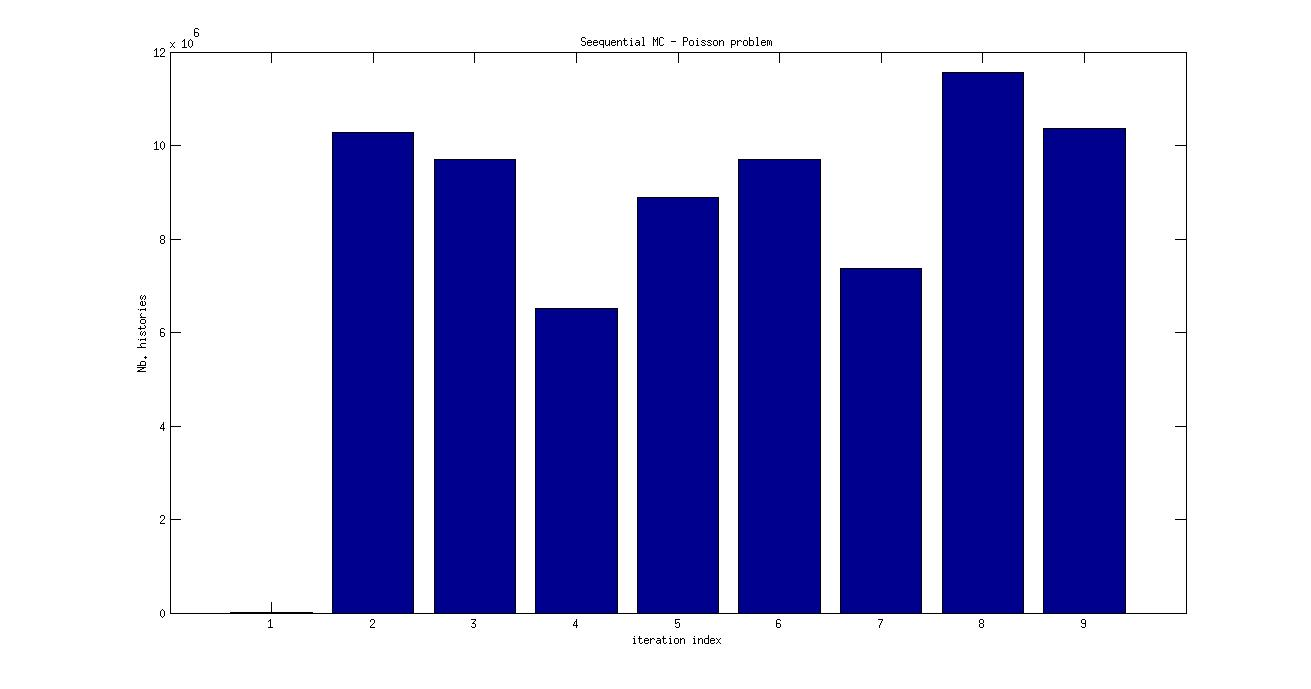
\includegraphics[width=\textwidth]{SEQ_poisson.jpg}
    \caption{Sequential MC - Poisson problem. Number of random walks employed
at each numerical iteration.}
\label{SEQ_poisson}
\end{figure}


\begin{figure}[h!]
  \centering
    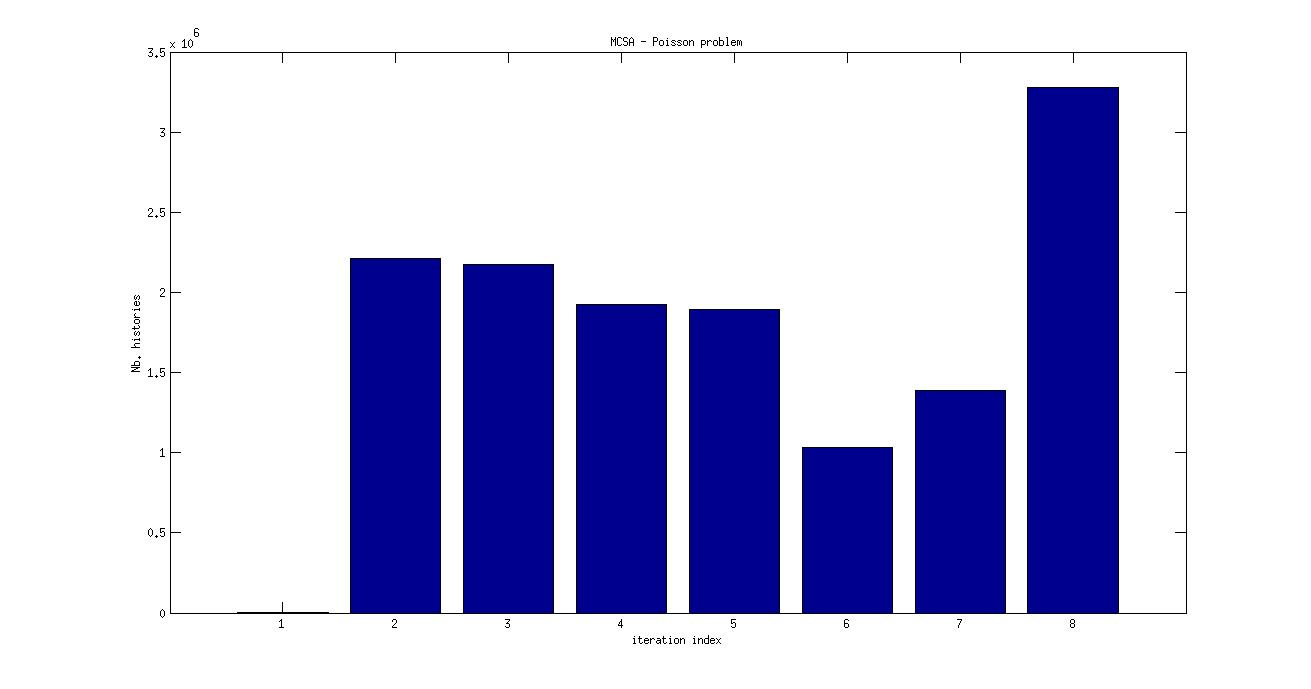
\includegraphics[width=\textwidth]{MCSA_poisson.jpg}
      \caption{MCSA - Poisson problem. Number of random walks employed at each
numerical iteration.}
\label{MCSA_poisson}
\end{figure}

\subsubsection{Reaction-Diffusion Problem}

By modifying the equation of the previous test case, we consider now
an advection reaction problem

\begin{equation}
\begin{cases}
 -\Delta u +\sigma u= f \quad \text{in}\quad \Omega \\
 u=0\quad \text{on} \quad \partial\Omega
 \end{cases}
\end{equation}
where $\Omega=(0,1)\times (0,1)$, $\sigma=0.1$ and $f=1$.
A finite difference scheme is applied to discretize the problem.
The number of nodes
on each direction of the domain is 100, so that $h\approx 0.01$. The
discretized problem has 9604 d.o.f's. A left
diagonal preconditioning is still applied to
the stiffness matrix obtained from the discretization. The 1-norm of the
iteration matrix is $\lVert H\rVert_1\approx 0.9756$. This automatically
guarantees the convergence of the Adjoint Monte Carlo linear solver. The
computation of the solution to the partial differential problem is still
accomplished with the MCSA algorithm. A threshold of $\varepsilon =10^{-8}$ is
used as a stop criterion for the relative residual. The threshold
for the adaptive selection of the random walks instead is set
to $\varepsilon_1=0.1$.
In Table \ref{DR_results} a comparison between the deterministic Synthetic
Acceleration
scheme, Sequential MC and the MCSA is provided.
The employment of the MCSA provides a significant reduction of the number of
histories necessary to satisfy the convergence criterion, in line with results
coming from the previous test case.

\begin{table}[!h]
\centering
\hspace*{-0.8cm}
\begin{tabular}{|c|c|c|c|}
\hline
algorithm & relative err.& \# iterations & average \# histories per iteration\\
\hline
 Synthetic acceleration & $9.073\cdot 10^{-8}$ & 634 & - \\
\hline
 Sequential MC & $8.415 \cdot 10^{-8}$ &  8 & 12,391,375\\
 \hline
 Adjoint MCSA & $6.633 \cdot 10^{-8}$ &  7 & 3,163,700\\
\hline
\end{tabular}
\caption{Numerical results for the diffusion reaction problem.}
\label{DR_results}
\end{table}


\begin{figure}[h!]
  \centering
    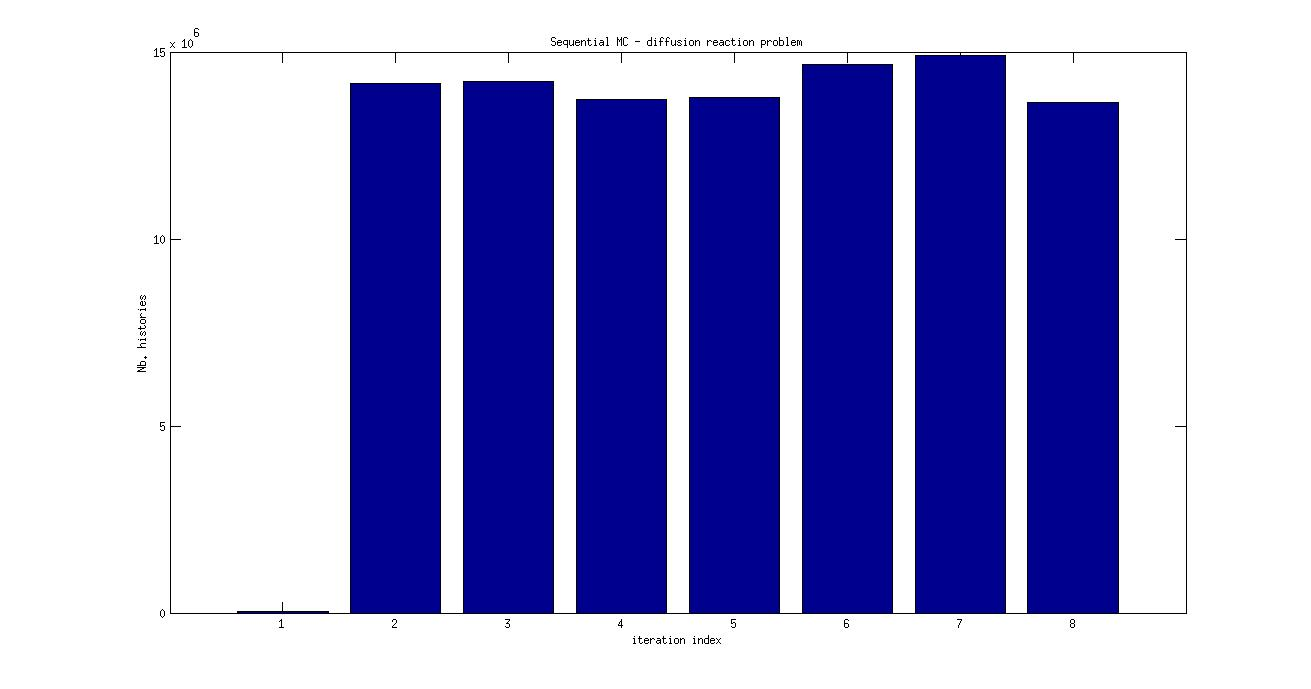
\includegraphics[width=\textwidth]{SEQ_diffreac.jpg}
      \caption{Sequential MC - Diffusion reaction problem. Number of random
walks
employed at each
numerical iteration.}
\label{SEQ_diffreac}
\end{figure}


\begin{figure}[h!]
  \centering
    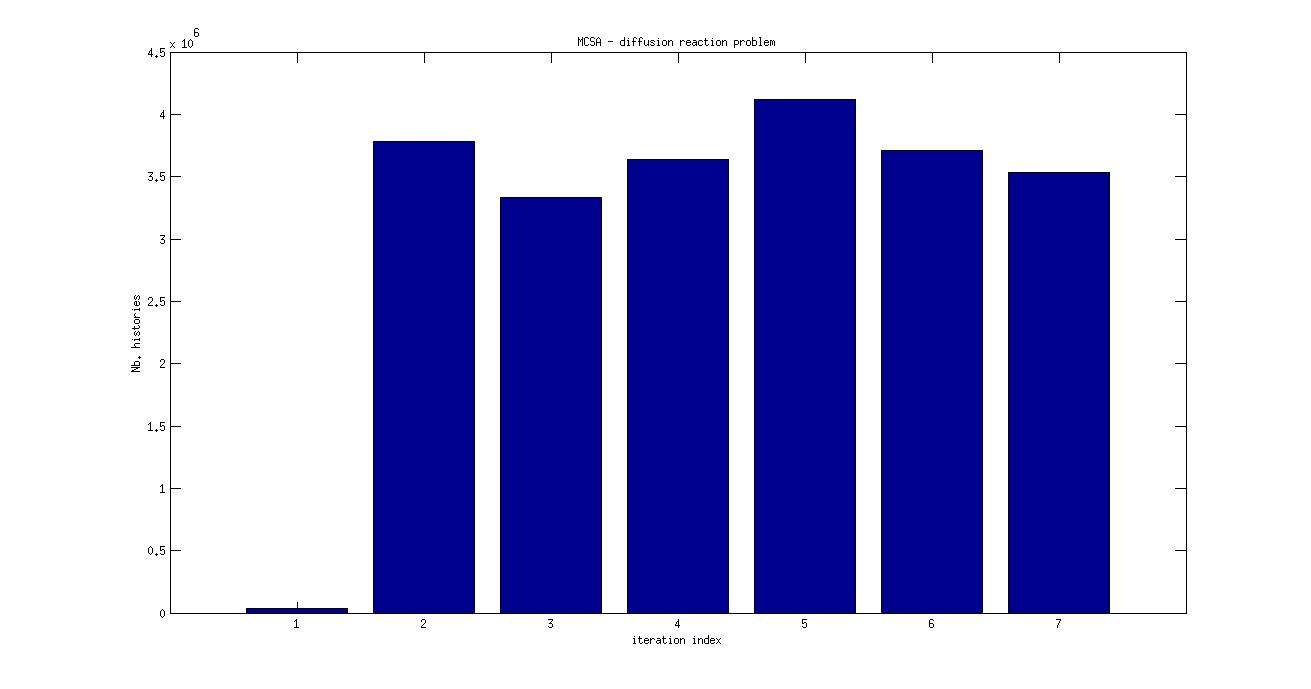
\includegraphics[width=\textwidth]{MCSA_diffreac.jpg}
      \caption{MCSA - Diffusion reaction problem. Number of random walks
employed at each
numerical iteration.}
\label{MCSA_diffreac}
\end{figure}

\subsubsection{Parabolic Problem}

In this subsection we restrict our treatise to the analysis of parabolic
partial
differential problems of the form
\begin{equation}
\begin{cases}
 \frac{\partial u }{\partial t} + \mathcal{L}(u)=f \quad \text{in} \Omega \\
\text{B.C.} \quad \text{on}\quad \delta \Omega.
\end{cases}
\label{parabolic}
\end{equation}

The partial derivative in time is discretized with finite differences, whereas
quadrilateral linear finite elements are employed for the space discretization.
Naming $N_h$ the number of d.o.f.'s associated with the finite element
discretization, the problem \ref{parabolic} turn into a fully discretized
problem such as:

\[
 \bigg (\frac{1}{\Delta t}M+A\bigg )(\mathbf{u}^{k+1}-\mathbf{u}^k)+A[\theta
\mathbf{u}^{k+1}+(1-\theta)\mathbf{u}^k]=\theta
\mathbf{f}^{k+1}+(1-\theta)\mathbf{f}^k,
\]

where $k$ is an index that goes with the time dimension.

By tuning the value of the parameter $\theta$ different numerical schemes can
be obtained with different properties of numerical stability.
However our discussion is not involved in this kind of issues.
In particular we restrict our attention to a single generic time step
associated with an Implicit Euler time discretization (corresponding to
$\theta=1$). The vector of the right hand side is chosen so that the exact
solution to the linear system for the specific time step chosen is a unit
vector $\tilde{\mathbf{u}}=\mathbbm{1}^{N_h}$.

By referring to $h$ as the space discretization step, we pick
\[
 \Delta t \le C h.
\]


Give an open and bounded set $\Omega=(0,1)\times(0,1)$, we consider the
following problem
\begin{equation}
 \begin{cases}\frac{\partial u}{\partial t} -\mu \Delta u
+\boldsymbol{\beta}(\mathbf{x})\cdot \nabla u=0, \;\; \quad \quad
\mathbf{x}\in \Omega,\quad t\in(0,T] \\
u(\mathbf{x},0) = u_0, \qquad \qquad \qquad \qquad \quad \mathbf{x}\in
\Omega \\
u(\mathbf{x},t)=u_D(\mathbf{x}),  \; \, \, \qquad \qquad \qquad \quad
\mathbf{x}\in \partial
\Omega, \quad t\in(0,T],
 \end{cases}
\end{equation}

where $\mu=\frac{3}{200}$, $\boldsymbol{\beta}(\mathbf{x})=[2y(1-x^2),\;
-2x(1-y^2)]^T$, \\$u_D=0$ on $\{\{x=0\}\times (0,1)\}$, $\{(0,1)\times
\{y=0\}\}$, $\{(0,1)\times \{y=1\}\}$.\newline

The discretization of the problem is realized with the \texttt{IFISS} toolbox.
The value of the discretization step is $h=2^{-8}$, generating a discretized
linear system with 66,049 d.o.f.'s.
As concerns the time discretization, the time step is set to $\Delta t =
10h$.\newline

The sparse approximate inverse is employed for
the linear system at hand as a right preconditioner, with a drop tolerance of
$\tau=0.05$ for both the factors.

In this situation it is not possible to
resort to any of the sufficient conditions to verify the convergence. Therefore
the only viable option is the explicit computation of the spectral radii of $H$
and $\hat{H}$.
The spectral radius of the iteration matrix is $\rho(H)\approx
0.9218$ and the spectral radius of $\hat{H}$ for the Adjoint Monte Carlo is
$\rho(\hat{H})\approx 0.9148$. The transition probability employed is the
Almost
Optimal one. Resorting to a Uniform Probability in this case would have impeded
the
convergence, since in this case $\rho(\hat{H})\approx 1.8401$.
Therefore
this is an example demonstrating that the Almost Optimal Probability
facilitates the performance of the stochastic algorithm, outperforming the
Uniform one.

The fill-in effect is
\[
 \frac{nnz(H)}{nnz(A)}=4.26,
\]
therefore the relative number of nonzero elements in $H$ is still acceptable
in terms of sparsity pattern and memory storage.

The threshold for the check on the relative residual is set to $\varepsilon
=10^{-8}$ is, whilst the threshold
for the adaptive selection of the random walks is set
to $\varepsilon_1=0.1$.
In order to test the effectiveness of employing the MCSA with respect to a
purely deterministic scheme, a comparison with the Richardson algorithm and
the Sequential Monte Carlo is
accomplished. The results are shown in Table \ref{parabolic_results}. As you
can see, the adoption of both Sequential Monte Carlo and MCSA reduces
dramatically the number of iterations with
respect to the fixed point method. Of course this
advantage has the
increase of the computational time as a payoff. Nevertheless we put off this
discussion which is of
interest for a parallelized implementation of the method. Even more the number
of random walks employed by the Sequential MC is higher than the one associated
with the MCSA, in accordance with the previous results.

\begin{table}[!h]
\centering
\hspace*{-0.8cm}
\begin{tabular}{|c|c|c|c|}
\hline
algorithm & relative err.& \# iterations & average \# histories per iteration\\
\hline
 Richardson & $6.277\cdot 10^{-7}$ & 178 & - \\
 \hline
 Sequential MC & $1.918 \cdot 10^{-9}$ & 8 & 51,535,375\\
\hline
 Adjoint MCSA & $1.341\cdot 10^{-9}$ & 6 & 16,244,000\\
\hline
\end{tabular}
\caption{Numerical results for the parabolic problem.}
\label{parabolic_results}
\end{table}


\begin{figure}[h!]
  \centering
    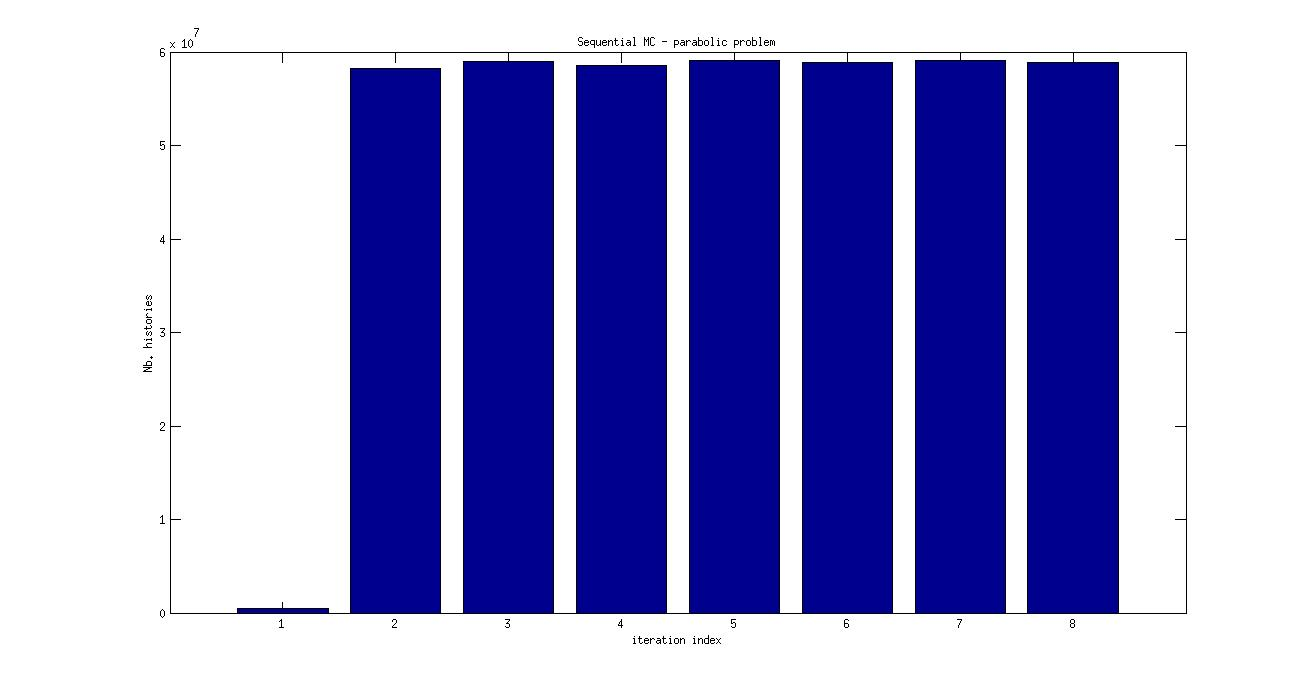
\includegraphics[width=\textwidth]{SEQ_parabolic.jpg}
      \caption{Sequential Monte Carlo - Parabolic problem. Number of random
walks
employed at each
numerical iteration.}
\label{MCSA_parabolic}
\end{figure}


\begin{figure}[h!]
  \centering
    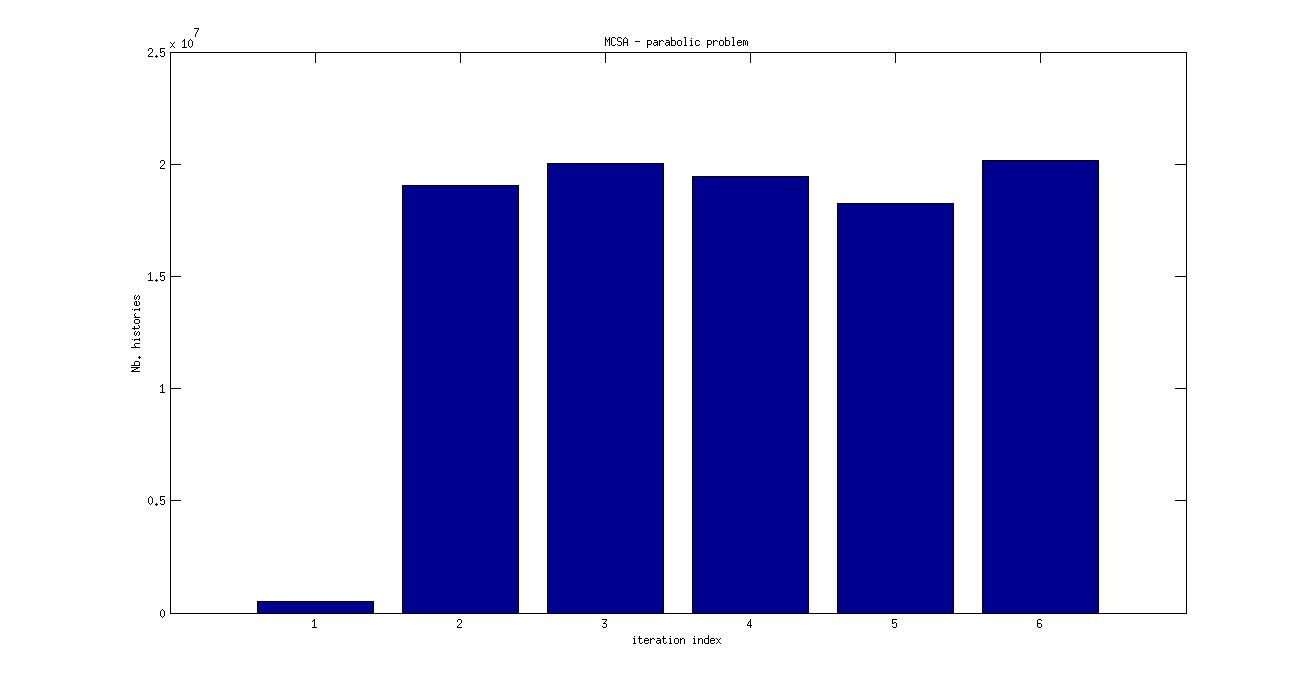
\includegraphics[width=\textwidth]{MCSA_parabolic.jpg}
      \caption{MCSA - Parabolic problem. Number of random walks
employed at each
numerical iteration.}
\label{MCSA_parabolic}
\end{figure}


\section{Conclusions and Future Work}

The work presented in this paper has been accomplished to provide an overview
about MC linear solvers. In particular the goal was to combine the main
theoretical results found in literature with additional novel contributions on
both the theoretical and empirical sides. This made it possible to understand
the actual limitations of the presented algorithms.

Necessary and sufficient conditions to ensure convergence are too costly for
most of the applicative problems coming fro engineering and Computational
Physics. On the other hand, sufficient criteria are currently viable for a
restricted set of matrices (generalized diagonally dominant).

An empirical analysis has been carries out on parabolic problems and it has
been shown that a proper selection of the time discretization step enables the
employment of stochastic solvers.

We reserve for future works the analysis of the plausible connections between
$\rho(H)$, $\rho(\hat{H})$ and the number of numerical iterations necessary to
reach convergence. Moreover a study about the resilience of the problem will be
accomplished, resorting to fault injection techniques.
i


\addcontentsline{toc}{chapter}{\refname}
\bibliographystyle{alpha}
\bibliography{library}
%\nocite{*}

\end{document}
